% Generated by research.render_springer_manuscript. Edit main_itt.tex.
% Working scientific draft; outstanding results are not supplied by rendering.
\documentclass[pdflatex,sn-basic]{sn-jnl}
\usepackage[T1]{fontenc}
\usepackage[utf8]{inputenc}
\usepackage{lmodern}
\usepackage{amsmath,amssymb,amsfonts}
\usepackage{graphicx,booktabs,array,tabularx}
\usepackage{microtype,xurl,tikz}
\usetikzlibrary{arrows.meta,positioning,fit}
\setlength{\emergencystretch}{2em}
\hypersetup{hidelinks,pdfauthor={},pdftitle={The Tourist Trap: Auditing Hard-Negative Reranking for Vietnamese Tourism Question Answering}}
\begin{document}
\title{The Tourist Trap: Auditing Hard-Negative Reranking for Vietnamese Tourism Question Answering}
\author{Anonymous for review}
\abstract{Reliable tourism question answering requires evidence that supports a requested
fact, rather than merely sharing its topic. We audit hard-negative augmentation
for a cross-encoder in a Vietnamese tourism retrieval pipeline. An archived
evaluation of nine checkpoints, covering three regimes and three seeds, uses
1,136 fixed positive--negative test pairs. Mean pairwise accuracy is
$0.8826\pm0.0008$ for the 7,618-pair baseline, $0.9654\pm0.0015$ after 525
additional adversarial pairs, and $0.9683\pm0.0014$ after 1,050 additions.
The augmented regimes are not statistically distinguishable in the reported
seed-wise paired comparisons. The data and code audit identifies defective
pairs, cross-role passage reuse despite disjoint document IDs, and legacy
settings that do not implement their advertised loss ablations. An 80-query
candidate-pool diagnostic motivates a transfer-failure hypothesis but uses
incomplete relevance judgments. A separate recovery audit maps two returned
second-round workbooks, each containing 268 questions and 1,688 passage reviews,
to a preserved 286-question development draft. These records do not finalize
later revised wording or establish corpus-wide unanswerability. The findings
support a bounded pairwise comparison and a reproducible account of outstanding
evaluation controls. They do not isolate adversarial hardness from data volume,
margin composition or training budget, and do not establish improved full-corpus
ranking or generated-answer faithfulness.}
\keywords{Retrieval-augmented generation , Hard negatives , Vietnamese tourism , Reranking , Evidence sufficiency}
\maketitle
\section{Introduction}
Tourism information supports decisions about when to visit, where to travel and
which services or conditions apply. A wrong date, place or eligibility condition
can change such a decision even when an answer sounds topically appropriate.
Retrieval-augmented generation (RAG) conditions generation on external
information \citep{lewis2020retrieval}, but an implementation that retrieves
relevant-looking passages does not automatically establish evidence sufficiency,
source faithfulness or the current validity of the information.

Recent tourism research already demonstrates several forms of language-model
assistance. ViTravelRAG addresses Vietnamese travel assistance and reports a
human-annotated VietnamTravel-VQA resource \citep{vitravelrag2026}; TRACE studies
sustainable conversational recommendations \citep{banerjee2026trace}. Work in
\emph{Information Technology \& Tourism} investigates semantically guided access
to real-time occupancy data, human-supervised hotel review assistance and audits
of LLM-assisted hotel selection
\citep{neubig2026occupancy,yoon2026hormas,baig2026hotelaudit}.
Consequently, applying RAG to tourism, using Vietnamese, or auditing an AI system
cannot by itself establish a new contribution. The specific evidence question
and its relation to tourism tasks must be demonstrated.

We examine one component of a Vietnamese tourism system: a cross-encoder that
scores query--passage pairs after hybrid candidate retrieval. The recorded
training regimes add domain-specific adversarial pairs to an unaugmented
baseline. Their reported checkpoint audit shows a large increase in the ability
to score a supplied positive above a supplied negative. This is a useful,
bounded finding. It is distinct from locating evidence in a corpus, choosing
among many plausible passages, or producing a supported answer. Those distinctions
are material because recent methods already address source-dependent shortcuts
in synthesized negatives, evidence utility and robust response selection
\citep{zhang2026causalneg,liu2026cormrag}.

The present investigation asks: (RQ1) how large and repeatable are the pairwise
differences between the recorded training regimes; (RQ2) which data and objective
properties qualify their interpretation; and (RQ3) what additional evidence is
required before transferring the result to tourism evidence selection and answer
generation? RQ3 motivates a development protocol and diagnostic analyses; it does
not supply a completed confirmatory end-to-end comparison.

The supported contributions are:
\begin{enumerate}
\item A checkpoint-level account of three recorded reranker regimes over three
seeds on one fixed test set, with paired comparisons and defective-pair
sensitivity analysis.
\item A data and code audit that distinguishes document-ID disjointness from
passage reuse, identifies ineffective legacy ablation settings, and separates
pairwise discrimination from candidate-pool evidence selection.
\item A versioned, source-grouped development workflow with independent review
records and explicit handling of revised questions and incomplete answerability
evidence. Its current output is a draft resource, rather than a validated public
benchmark or a new annotation methodology.
\end{enumerate}
These contributions concern reproducibility and the evidential limits of one
tourism retrieval study. A new loss, state-of-the-art ranking, the first Vietnamese
tourism dataset and reduced hallucination are not claimed.

\section{Related Work}
\subsection{Hybrid retrieval and multilingual reranking}
BM25 provides lexical relevance signals \citep{robertson2009bm25}, while
M3-Embedding supplies multilingual retrieval representations \citep{baai2024bgem3}.
Reciprocal rank fusion combines ranked lists without calibrating their raw
scores \citep{cormack2009rrf}. These established components describe the system;
their combination is not a new retrieval algorithm. The initial cross-encoder
is the released \texttt{BAAI/bge-reranker-base} checkpoint. Its model repository
is a software provenance source, rather than a peer-reviewed research citation.

\subsection{Hard negatives and evidence utility}
CausalNeg studies source-dependent shortcuts and a generative--discriminative
gap when synthesized hard negatives are used to train dense retrievers
\citep{zhang2026causalneg}. Our cross-encoder and supplied-pair protocol differ
from that setting. However, the general observation that synthesized negatives
can harm retrieval is not a new contribution of this study.
CoRM-RAG trains an Evidence Critic for decision-supporting evidence under query
perturbations, including false premises, and studies risk-aware abstention
\citep{liu2026cormrag}. Thus the distinction between semantic relevance and
answer utility has prior methodological treatment. A domain-specific audit must
establish what its additional evidence shows, rather than rename that distinction.

\subsection{Tourism resources and application evidence}
ViTravelRAG addresses multimodal Vietnamese travel assistance. Its publisher
abstract reports 1,000 human-annotated query--document pairs
\citep{vitravelrag2026}; the underlying data were not independently inspected here.
Consequently, this project cannot claim the first Vietnamese tourism RAG system
or dataset. TRACE concerns sustainable recommendations and counterfactual
travel alternatives \citep{banerjee2026trace}. Those alternatives differ from
factually incorrect premises in passage-grounded questions, and its recommendation
outcomes are not directly comparable with pairwise discrimination accuracy.

Recent articles in \emph{Information Technology \& Tourism} study semantically
guided access to occupancy data, a human-supervised hotel review assistant, and
an audit of reputation signals in LLM-assisted hotel selection
\citep{neubig2026occupancy,yoon2026hormas,baig2026hotelaudit}. They illustrate
application and audit contributions tied to specific tourism information needs.
They do not establish that the present reranker improves visitor decisions,
operational efficiency or generated-answer faithfulness. These outcomes require
separate task definitions and measurements.

\section{Methodology}
\subsection{System Overview}
Figure~\ref{fig:framework} separates the recorded pair-training branch from the implemented online retrieval and generation architecture. The checkpoint table evaluates supplied passage pairs; the figure does not imply that those scores validate every stage of the architecture.

\begin{figure}[htbp]
\centering
\resizebox{\linewidth}{!}{%
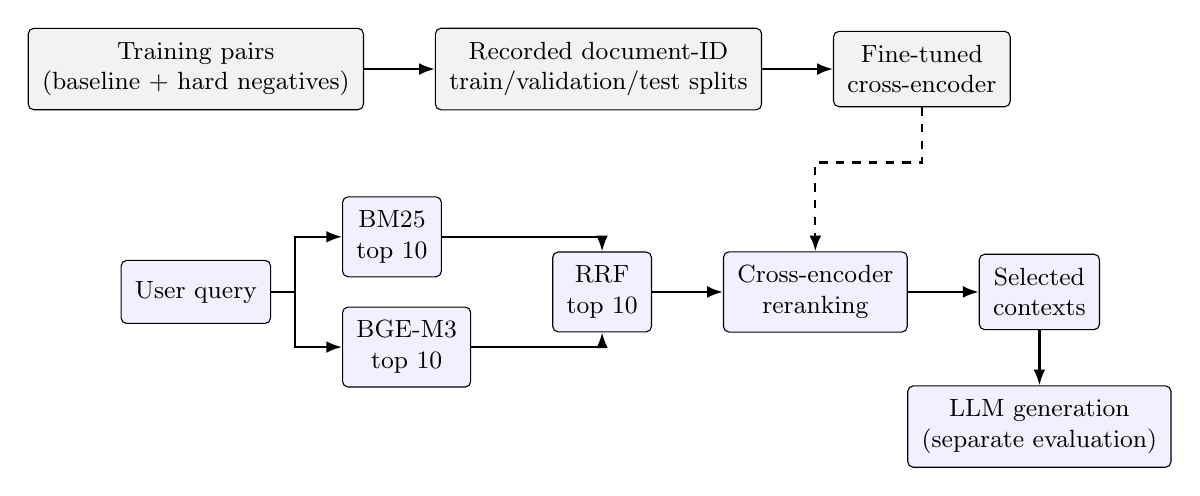
\begin{tikzpicture}[
  >=Latex, font=\small,
  node distance=7mm and 9mm,
  unit/.style={draw,rounded corners=2pt,align=center,inner sep=5pt,minimum height=8mm},
  train/.style={unit,fill=black!5},
  online/.style={unit,fill=blue!6},
  arrow/.style={-{Latex[length=2.0mm]},thick}
]
\node[train] (pairs) {Training pairs\\(baseline + hard negatives)};
\node[train,right=of pairs] (split) {Recorded document-ID\\train/validation/test splits};
\node[train,right=of split] (model) {Fine-tuned\\cross-encoder};
\draw[arrow] (pairs)--(split);
\draw[arrow] (split)--(model);
\node[online,below=19mm of pairs] (query) {User query};
\node[online,right=of query,yshift=7mm] (bm) {BM25\\top 10};
\node[online,right=of query,yshift=-7mm] (dense) {BGE-M3\\top 10};
% The next row is independent of the offline training connection.
\node[online,right=14mm of bm,yshift=-7mm] (rrf) {RRF\\top 10};
\node[online,right=of rrf] (rerank) {Cross-encoder\\reranking};
\node[online,right=of rerank] (context) {Selected\\contexts};
\node[online,below=of context] (gen) {LLM generation\\(separate evaluation)};
\draw[arrow] (query.east) -- ++(3mm,0) |- (bm.west);
\draw[arrow] (query.east) -- ++(3mm,0) |- (dense.west);
\draw[arrow] (bm.east) -| (rrf.north);
\draw[arrow] (dense.east) -| (rrf.south);
\draw[arrow] (rrf)--(rerank);
\draw[arrow] (rerank)--(context);
\draw[arrow] (context)--(gen);
\draw[arrow,dashed] (model.south) -- ++(0,-7mm) -| (rerank.north);
\end{tikzpicture}%
}
\caption{Conceptual architecture. The numerical results verified in this paper concern the offline-trained cross-encoder evaluated on fixed pairs; the online retrieval and generation stages are not established by those pairwise numbers.}
\label{fig:framework}
\end{figure}

\subsection{Tourism Corpus and Candidate Retrieval}
The audited corpus snapshot contains 56,984 chunks, 4,122 distinct source
URLs and 6,200 internal document IDs. URL counts and internal IDs are different
units and should not be interpreted as conflicting article counts. The processing
configuration records nominal chunk size 600 and overlap 100; these values are
not asserted to be transformer-token counts. Vietnamese segmentation and lexical
normalization support BM25-style search. The implementation uses 1,024-dimensional
BGE-M3 dense vectors, L2 normalization and a FAISS \texttt{IndexFlatIP} index.
These are implementation settings, not a new full-system performance result.

For a query $q$, both lexical and dense search return an ordered candidate list. RRF aggregates ranks, for a document $d$ in the union of the lists, as
\begin{equation}
\operatorname{RRF}(d\mid q)=\sum_{j\in\{\mathrm{BM25},\mathrm{dense}\}:\ d\in R_j(q)}\frac{1}{k+\operatorname{rank}_j(d\mid q)},\qquad k=60.
\label{eq:rrf}
\end{equation}
Missing candidates contribute no term to the sum. The operational pipeline uses a top-10 candidate pool followed by cross-encoder reranking and a nominal top-3 context window for generation. These parameters describe the system implementation, not the evaluation scope of Table~\ref{tab:main}.

\subsection{Pair Construction, Training Regimes and Loss}
Let $q_i$ be a query, $d_i^+$ a positive passage and $d_i^-$ a negative passage. The cross-encoder produces scalar logits $s(q_i,d_i^+)$ and $s(q_i,d_i^-)$. The training implementation computes
\begin{align}
\Delta_i &= s(q_i,d_i^+)-s(q_i,d_i^-),\\
\alpha_i &= \sigma(-\Delta_i),\\
\mathcal{L}_{\mathrm{weighted}} &= \frac{1}{B}\sum_{i=1}^B
\max\!\left(0,m_i-\Delta_i\right)\left(1+\alpha_i\right).
\label{eq:actual_loss}
\end{align}
Here $m_i$ is the \emph{sample-specific margin read from each training record}, and $B$ is the mini-batch size. The code does not enforce a universal fixed margin of 2.0 for the main Full-Trap regime. The sigmoid factor modifies optimization, but the available experiments do not isolate its causal contribution against unweighted margin ranking loss. We therefore treat Eq.~\eqref{eq:actual_loss} as an \emph{implementation description}, not as a validated gain attributable to adaptive weighting.

The baseline training file has 7,618 pairs; the second file has 8,143 pairs after 525 additional adversarial pairs; the third has 8,668 pairs after 1,050 additions. Historic experiment names call these \emph{0\%, 6.85\%, and 13.7\%}, respectively. These names are retained as checkpoint identifiers only. Under the standard fraction-of-current-training-set definition, the added-pair fractions are $525/8{,}143=6.45\%$ and $1{,}050/8{,}668=12.11\%$; the historic labels must not be interpreted as those fractions.

The underlying sample margins were inspected directly: 3,799 records have $m_i=0.5$, 3,819 have $m_i=1.2$, and the augmented dataset contributes 525 or 1,050 additional records with $m_i=2.0$. An experiment changing only the function's \texttt{default\_margin} cannot alter these stored values, because the training loader reads the record's existing \texttt{margin} field first.

\subsection{Pairwise Metrics and Statistical Testing}
Each held-out item contains exactly one positive and one negative. Pairwise accuracy uses a strict comparison, so ties count as incorrect:
\begin{equation}
A=\frac{1}{N}\sum_{i=1}^N\mathbb{I}\!\left[s(q_i,d_i^+)>s(q_i,d_i^-)\right],\qquad N=1{,}136.
\label{eq:accuracy}
\end{equation}
For a two-item list with one relevant item, rank is 1 for a correct strict comparison and 2 otherwise; under the evaluation's tie convention, the other metrics are deterministic functions of $A$:
\begin{equation}
\mathrm{P@1}=A,\quad \mathrm{MRR@2}=\frac{1+A}{2},\quad
\mathrm{NDCG@2}=A+\frac{1-A}{\log_2(3)}.
\label{eq:metric_identity}
\end{equation}
Consequently, the three metric columns must not be interpreted as independent tests of corpus-scale retrieval quality. They summarize the same pairwise outcomes.

The archived nine-checkpoint audit retained here re-evaluated the checkpoints using the fixed test JSON (SHA-256 prefix \texttt{473d43d8376ba6ab}; the full digest is retained in the audit manifest), with maximum sequence length 512, fixed-length padding, CUDA BF16 inference, and batch size one. Correctness was independently recomputed from exported positive and negative logits. We report the mean and \emph{population} standard deviation ($\mathrm{ddof}=0$) over seeds 42, 123 and 999, to match the diagnostic report. Exact two-sided McNemar tests use query-matched binary correctness masks for a specified seed \citep{mcnemar1947note}. A difference in such a test does not directly establish better generated answers.

\section{Experimental Materials and Data Quality}
\subsection{Dataset and Split Overview}
\begin{table}[htbp]
\centering
\caption{Audited experimental inventory. Corpus counts were checked against the project CSV snapshot; pair counts and test integrity were checked against the supplied files. The nine-checkpoint scores are retained from the archived audit.}
\label{tab:inventory}
\begin{tabular}{lr}
\toprule
Item & Value\\\midrule
Distinct source URLs & 4,122\\
Internal corpus document IDs & 6,200\\
Corpus chunks & 56,984\\
Baseline training pairs & 7,618\\
Half-Trap training pairs (additional) & 8,143 (525)\\
Full-Trap training pairs (additional) & 8,668 (1,050)\\
Validation pairs & 1,033\\
Fixed test pairs & 1,136\\
Unique test \texttt{doc\_id} groups & 247\\
Seed/checkpoint combinations & $3\times3=9$\\
\bottomrule
\end{tabular}
\end{table}

The recorded workflow used semantic near-duplicate filtering and a document-grouped train/validation/test partition. Prior audit logs reported no shared grouping IDs across partitions, but also flagged cross-role reuse of passage text between positive and negative roles. These claims refer to different leakage mechanisms. A zero document-ID intersection is not proof that all textual contamination or near-duplicate leakage has been eliminated. Exact split provenance and overlap rules should accompany any final release.

\subsection{Passage reuse, corpus mapping and training-pair defects}
Exact NFC/whitespace-normalized checks found no shared query or document-ID
values across train, validation and test. However, 999 of the 1,136 test positives
occur in training negatives (146 distinct texts), and 793 test negatives occur
in training positives (536 distinct texts). Relevance is query-dependent, so
cross-role reuse is not automatically a contradictory label or proof of causal
inflation. It does show that passage-level disjointness does not follow from
the document-ID split.

Exact corpus lookup maps 118 test positives uniquely and 11 to multiple chunks;
1,007 have no exact match. This does not prove that equivalent supporting
evidence is absent. It does mean that supplied pair labels cannot be treated
as corpus-level relevance judgments. The distinction is especially important
when interpreting a candidate-pool evaluation.

\begin{table}[htbp]
\centering
\caption{Mechanical pair defects in the supplied datasets. Counts across nested
training files are not counts of distinct underlying defective examples.}
\label{tab:pairquality}
\begin{tabular}{lrrr}
\toprule
Dataset & Rows & Identical positive/negative & Empty negative\\
\midrule
B training & 7,618 & 0 & 0\\
C training & 8,143 & 70 & 1\\
D training & 8,668 & 123 & 1\\
Validation & 1,033 & 27 & 0\\
Test & 1,136 & 7 & 1\\
\bottomrule
\end{tabular}
\end{table}
The original data are retained. Table~\ref{tab:pairquality} is a review ledger,
not an automatically cleaned training set or a replacement test benchmark.

\subsection{Test Integrity and Sensitivity Protocol}
The fixed test includes seven rows where the positive and negative passages are exactly identical (zero-based indices 1008, 1014, 1018, 1019, 1079, 1087 and 1088), plus one row with an empty negative (index 1047). This represents eight problematic rows, or approximately 0.70\% of the original test. Identical-text pairs cannot be distinguished from their text alone. For backward compatibility and auditability, we retain all 1,136 items in the primary results and separately report a post-hoc sensitivity calculation on the remaining 1,128 items. This filtered analysis must not be presented as a replacement pre-registered benchmark.

Queries share document sources (247 unique \texttt{doc\_id} groups), so query-level confidence tests may understate uncertainty when within-source outcomes are correlated. Exploratory source-group bootstrap results are therefore presented only as a diagnostic supplement.

\section{Results}
The checkpoint results below are retained from the archived audit, not newly
executed measurements in this revision. Dataset integrity and the returned
review workbooks were checked separately. No current full-corpus or
generated-answer improvement is inferred from the archived pairwise table.

\subsection{Archived Pairwise Discrimination}
\begin{table}[htbp]
\centering
\caption{\textbf{Archived checkpoint-audit results} on 1,136 fixed positive--negative test pairs (mean $\pm$ population SD over three seeds). MRR@2 and NDCG@2 are derived from pairwise outcomes as in Eq.~\eqref{eq:metric_identity}.}
\label{tab:main}
\footnotesize
\setlength{\tabcolsep}{5pt}
\begin{tabular}{lccc}
\toprule
Training condition & Pairwise accuracy & MRR@2 & NDCG@2\\\midrule
B: baseline (7,618) & $0.8826\pm0.0008$ & $0.9413\pm0.0004$ & $0.9567\pm0.0003$\\
C: +525 hard negatives & $0.9654\pm0.0015$ & $0.9827\pm0.0007$ & $0.9872\pm0.0006$\\
D: +1,050 hard negatives & $\mathbf{0.9683\pm0.0014}$ & $\mathbf{0.9842\pm0.0007}$ & $\mathbf{0.9883\pm0.0005}$\\
\bottomrule
\end{tabular}
\end{table}

Table~\ref{tab:main} retains the re-inference figures reported in the preserved author-supplied audit. This revision checks their aggregate arithmetic but does not repeat checkpoint inference. The underlying nine-model raw score package remains necessary for independent reproduction. Relative to B, C increases mean pairwise accuracy by 8.27 percentage points and D by 8.57 percentage points. The mean advantage of D over C is only 0.29 percentage points. The regimes also differ in sample count, margin composition and potentially the number of optimizer updates under an epoch-based schedule; these results do not isolate adversarial hardness from those changes. Compared with B, D increases MRR@2 by approximately 4.55\% and NDCG@2 by approximately 3.31\% \emph{in relative terms}; these are transformations of the pairwise-accuracy improvement, not evidence of improved full-corpus ranking.

\subsection{Seed-wise Results and Paired Significance}
\begin{table}[htbp]
\centering
\caption{Accuracy by seed and exact paired McNemar tests for seed 42.}
\label{tab:seedwise}
\footnotesize
\begin{tabular}{lrrr}
\toprule
Condition & Seed 42 & Seed 123 & Seed 999\\\midrule
B & 0.882042 & 0.882042 & 0.883803\\
C & 0.964789 & 0.963908 & 0.967430\\
D & 0.968310 & 0.966549 & 0.970070\\
\bottomrule
\end{tabular}\quad
\begin{tabular}{lr}
\toprule
Seed-42 comparison & Exact $p$\\\midrule
B vs C & $2.315\times10^{-21}$\\
B vs D & $1.493\times10^{-23}$\\
C vs D & $0.4545$\\
\bottomrule
\end{tabular}
\end{table}

For seed 42, the B--C contingency counts (both correct, B only, C only, both wrong) were $(993,9,103,31)$; for B--D, $(995,7,105,29)$; and for C--D, $(1090,6,10,30)$. Thus the B--C and B--D differences are significant in query-level exact McNemar tests, but C--D is not. C--D is also non-significant when evaluated separately at seed 123 ($p=0.6776$) and seed 999 ($p=0.6291$). No evidence from these tests establishes that the larger augmented set is superior to the smaller one.

The training-time and re-inference logs differ by a small number of individual predictions for B and C. The original stored correctness masks were unavailable in the audit package, so their differences cannot yet be attributed to BF16 batch formation or other implementation details. We use the reproducible score-file results consistently instead of combining the old contingency matrix with the new averages.

\subsection{Sensitivity to Invalid Test Pairs}
\begin{table}[htbp]
\centering
\caption{Post-hoc data-quality sensitivity analysis. Both columns are mean pairwise accuracy over the same three checkpoints per condition.}
\label{tab:sensitivity}
\begin{tabular}{lcc}
\toprule
Condition & Original $N=1{,}136$ & Excluding 8 flagged, $N=1{,}128$\\\midrule
B & 0.8826 & 0.8880\\
C & 0.9654 & 0.9713\\
D & 0.9683 & 0.9743\\
\bottomrule
\end{tabular}
\end{table}

The same ordering is observed after excluding the eight flagged cases (Table~\ref{tab:sensitivity}). This is a robustness check on the reported arithmetic, not grounds to redefine the test set without a documented protocol. Exploratory bootstrap resampling of the 247 source groups, averaged across the existing three seeds, yielded a 95\% percentile interval of approximately $[-0.00089,0.00692]$ for the D--C accuracy difference. It includes zero and is not a substitute for external evaluation.

\subsection{Legacy Training Runs: Audit of Ablation Labels}
The original manuscript labeled several experiments as constant-margin or ``alpha-off'' ablations. A code-level inspection revealed that the loader executes \texttt{item.get("margin", default\_margin)} while every training record supplies \texttt{margin}. Consequently, changing the default value in runs 4, 5 or 7 did not implement the advertised constant margin. Likewise, in runs 8 and 10, $\alpha=\sigma(-\Delta_i)$ is computed inside \texttt{torch.no\_grad()} but the objective still multiplies the hinge loss by $(1+\alpha)$. Those runs detach gradients through the weighting function; they do \emph{not} remove the weighting term.

\begin{table}[htbp]
\centering
\caption{\textbf{Archived training-log results, not valid controlled margin or loss ablations.} These rows are retained for transparent reporting, not evidence of a causal effect of the nominal setting. Their metrics have \emph{not} been independently re-inferred in the present checkpoint audit.}
\label{tab:legacy}
\footnotesize
\begin{tabularx}{\linewidth}{@{}lXcc@{}}
\toprule
Run & Actual interpretable change / warning & Logged acc. & Logged MRR\\\midrule
3 & Sample-specific margin, three epochs (reference) & $0.9683$ & $0.9842$\\
4 & Nominal default $0.5$; stored sample margins override it & $0.9712$ & $0.9856$\\
5 & Nominal default $1.0$; stored sample margins override it & $0.9718$ & $0.9859$\\
7 & Nominal default $3.0$; stored sample margins override it & $0.9695$ & $0.9847$\\
8 & Three epochs; detached sigmoid weight, not alpha removal & $0.9698$ & $0.9849$\\
9 & Five-epoch schedule; sigmoid weight retained & $0.9712$ & $0.9856$\\
10 & Five-epoch schedule; detached sigmoid weight retained & $0.9689$ & $0.9844$\\
\bottomrule
\end{tabularx}
\end{table}

The differences among these archived runs cannot support claims that a fixed margin of 1.0 is optimal, that switching off alpha reduces accuracy, or that the proposed weighted loss beats standard margin ranking loss. A valid controlled comparison will require explicitly overriding and logging the effective per-sample margin and comparing otherwise identical training configurations with and without sigmoid weighting.

\subsection{Exploratory Downstream Diagnostics (Not a Confirmatory Evaluation)}
An archived diagnostic on 80 validation queries compares models within identical
RRF candidate pools (Table~\ref{tab:pool80}). The designated exact gold chunk
appears in the pool for 57 queries. The augmented checkpoints place that exact
chunk in the top three less often than B. These are validation diagnostics with
one proxy gold chunk, incomplete relevance judgments and unreplayed model
provenance in the current revision. Other passages may also supply an answer.
The table therefore motivates a transfer hypothesis; it is not a confirmatory
estimate of answer quality or a causal demonstration that augmentation harms it.

\begin{table}[htbp]
\centering
\caption{Archived 80-query validation diagnostic using the same RRF pool for each
model. Counts refer to one designated exact gold chunk; they are not exhaustive
relevance judgments or a new held-out benchmark.}
\label{tab:pool80}
\begin{tabular}{lrrr}
\toprule
Condition & Gold in pool & Exact gold at 3 & Exact-gold MRR@10\\
\midrule
RRF order & 57/80 & 42/80 & 0.3914\\
B & 57/80 & 56/80 & 0.6365\\
C & 57/80 & 8/80 & 0.1390\\
D & 57/80 & 6/80 & 0.1435\\
\bottomrule
\end{tabular}
\end{table}

A previously generated 10-query downstream pilot, with draft rather than independently validated annotations, reported behavior success rates of 0.70 for RRF-only A, 0.80 for baseline reranker B, 0.40 for C and 0.20 for D. Reported exact-gold-at-3 values were 0.70, 0.70, 0.30 and 0.20, respectively. This pilot is too small and insufficiently validated to estimate production effectiveness or support formal significance claims. Nevertheless, it raises a concrete hypothesis of \emph{pairwise-to-candidate-set transfer failure}: a model that reliably distinguishes the supplied pair may still rank the correct corpus passage below other retrieved documents.

Separately, a 30-query exploratory answer-faithfulness scoring record, using a locally configured Qwen2.5-14B generator, reported behavior success of 7/30 for RRF versus 8/30 with a reranker (paired exact McNemar $p=1$). Its mean context-faithfulness values were approximately 0.422 versus 0.374. These values originated in a scoring workflow with proxy gold evidence and an NLI score carried forward from an earlier version; they are not independently human-validated results. We therefore refrain from using them as evidence that the trained reranker reduces hallucinations.

\section{Development of a Source-Grounded Tourism Evaluation}
\label{sec:development}
This section reports a development and annotation record, not model performance
on a new benchmark. It is separate from the fixed 1,136-pair test and the archived
diagnostics above. None of its pending labels replaces the historical test.

\subsection{Source grouping and evidence labels}
The preparation workflow canonicalizes source URLs and connects shared document
IDs and exactly normalized passage text. It forms 3,135 source components from
4,122 URLs. Known legacy training exposure, including passage use in negative
roles, is restricted to training; known evaluation-only exposure is excluded
from the new held-out partitions. Unknown provenance and semantic paraphrases
remain limitations. The initial draft samples 25 source families in each of
train, validation, calibration and test, producing 300 questions from 100
families. These are development allocations, not 300 independent test questions.

The proposed behaviors are answering a supported request, correcting a premise
contradicted by evidence, and declining when the declared evidence scope is
insufficient. Passage grades distinguish unrelated evidence (0), relevant but
insufficient context (1), and sufficient support (2). A question can have multiple
sufficient passages. Literal quotes are checked against their identified chunks;
matching text alone cannot establish semantic sufficiency or truth outside the
source. Answer-supporting evidence that crosses a source partition triggers
partition review, rather than relabeling relevant text as irrelevant.

\subsection{Recorded independent review and unresolved validity}
Two reviewers completed separate, opaque-ID workbooks covering the same 300
questions and 492 query--passage pairs. The research team confirmed that the
reviews were conducted independently. Recorded behavior labels, quality decisions
and relevance grades agree on every matched item, yielding nominal Cohen's
$\kappa=1.0$ for each categorical task \citep{cohen1960agreement}. The returned free-text responses,
rewrites and notes also match after normalization; this is retained in the audit.
Reviewer qualifications and procedural documentation must accompany a final
release. Agreement is a property of the recorded judgments and is not a
certificate of benchmark validity or a user study of tourism decisions.

Both reviewers propose keeping 134 questions, revising 152 and excluding 14.
Among the proposed rewrites, 93 still refer to an unspecified excerpt/position
and 59 retain an ellipsis. All 100 proposed refusals use a student-benefit
question pattern and currently record source-level absence, not a validated
corpus-wide evidence search. A same-URL check of 5,020 source passages finds two
additional student/benefit keyword passages for one question; they remain
unlabeled because co-occurrence is not sufficient evidence of eligibility.

\begin{table}[htbp]
\centering
\caption{Current development status. Review decisions apply to the original
wording; revised questions and reset qrels do not inherit approval.}
\label{tab:development}
\begin{tabularx}{\linewidth}{@{}l r >{\raggedright\arraybackslash}X@{}}
\toprule
Material or operation & Count & Status\\
\midrule
Original development questions & 300 & 100 source families; 75 questions per partition\\
Passage pairs reviewed per person & 492 & Original-query judgments recorded\\
Keep / revise / exclude proposals & 134 / 152 / 14 & Decisions on the original draft\\
Questions in the revised draft & 286 & Not frozen for model evaluation\\
Proposed rewritten questions & 156 & 93 information requests and 63 premise checks; pending review\\
Qrel rows in the revised ledger & 476 & Changed-query grades reset; not 476 newly approved pairs\\
New BM25 candidates & 14,300 & Top 50 for each draft query; unlabeled\\
\bottomrule
\end{tabularx}
\end{table}

The revised draft archives the 14 exclusions and proposes 156 assistant-written
rewrites: the 152 requested revisions plus four additional correction cases
identified during source inspection. Eight records move to a more informative
chunk within the same URL, source component and partition. Changed questions
lose their old approval, reference and search notes; their qrel grades are reset
while prior judgments are retained in the lineage. These proposals have not
received a new human approval and must not be described as human-validated data.

Checks against all 56,984 chunks find no cross-partition token-five-gram Jaccard
matches at threshold 0.65 for the 104 current anchors. This is a selected-anchor
lexical check, not proof of complete semantic decontamination. The revision also
flags 88 questions for tourism-task relevance, 13 counterfactuals involving
approximate quantities and five involving ranges. For example, a source stating
``more than 20 million'' does not necessarily contradict ``more than 21 million''.
A change of numeral can be unsupported without being demonstrably false.

\subsection{Recovered second-round review records}
A separate recovery audit binds the two returned second-round workbooks to the
preserved 286-question draft by unique exact normalized query wording, anchor
text and source URL. Each file contains 268 question records and 1,688 passage
records; all bind to the preserved corpus without altered passage text. The
original second-round opaque-ID mapping was unavailable, so this is a documented
text-identity recovery rather than a verification against the original export.
Eighteen questions in this draft have no corresponding returned question row.
This does not establish their status in any later, unavailable revision.

Both returned files record 93 \texttt{answer}, 72 \texttt{correct} and
103 \texttt{unclear} judgments. R01 records 259 \texttt{KEEP} and nine
\texttt{REVISE} decisions; R02 records 265 and three, respectively. Their
passage grades agree on 1,662 of 1,688 pairs. The latest R02 file was returned
after feedback; these descriptive comparisons are not a fresh blind reliability
estimate. A literal-quote check passes for all returned positive-grade rows,
but cannot establish semantic sufficiency or corpus-wide unanswerability.
No disagreements or incomplete records are automatically adjudicated, and no
human approval is transferred to later assistant-written wording.

\subsection{Requirements before a confirmatory evaluation}
The uniform refusal template must be diversified to avoid a question-style
shortcut. Information needs should be tied to an identified audience, such as
visitors or destination-information staff; historical management statistics
should be analyzed separately from visitor decisions. Corpus-scope refusals
require documented BM25, dense/RRF and source-neighbor review. Questions changed
in wording or factual target require an appropriate evidence recheck.

Once those conditions are met, the benchmark version, source partitions,
calibration procedure and primary outcomes can be frozen before test inference.
Risk--coverage and unsupported-answer rates must be reported alongside correct
answers and incorrect refusals. The current draft and candidate-mining counts
supply preparation artifacts, not evidence that such a system already succeeds.

\section{Discussion}
\subsection{The supported effect and its causal limits}
The strongest numerical finding is the repeatable pairwise difference between
the archived unaugmented and augmented regimes. The largest mean difference is
8.57 percentage points, while the smaller C--D difference remains statistically
unestablished. Because the regimes also change sample count and margin
composition, the audit does not isolate an effect of adversarial hardness, the
sigmoid multiplier, or additional optimization steps.

This is compatible with recent evidence that negative construction and training
distributions can matter substantially \citep{zhang2026causalneg}.
It neither validates a universal remedy nor explains the candidate-pool
observations by source shortcuts alone. A mechanistic claim requires matched
controls and an independently reviewed evidence task.

\subsection{From pairwise discrimination to evidence selection}
The three two-candidate metrics encode the same binary outcomes. Their numerical
agreement cannot corroborate corpus-scale retrieval. The low exact mapping of
legacy positives to the corpus also prevents treating this test as a full-corpus
relevance benchmark. The 80-query diagnostic uses different, validation-selected
queries and incomplete judgments, so its scores cannot be directly subtracted
from the fixed-test accuracy to estimate a transfer penalty.

A valid follow-up should distinguish four situations: known sufficient evidence
is absent from the candidate pool; it is present but selected poorly; selected
evidence is sufficient but the generator responds incorrectly; or the declared
knowledge source lacks sufficient reviewed evidence. Refusing despite available
support is a separate error. This decomposition is motivated by established
work on evidence utility and selective responses
\citep{liu2026cormrag}; applying it to the current
Vietnamese tourism artifacts remains an empirical task.

\subsection{Tourism relevance and the potential resource contribution}
The development workflow adds traceability and an explicit record of quality
problems, but a released resource needs more than scraped volume, changed
numerals and perfect recorded agreement. ViTravelRAG already reports Vietnamese
travel QA data \citep{vitravelrag2026}. The contribution to pursue is a
well-defined evidence task with useful source-linked labels and reproducible
controls, rather than a general language/domain priority claim.

The application question should identify who needs the information and what a
mistake changes. For visitors this may involve event timing, access or eligibility;
for destination staff it may involve retrieving correctly scoped historical
information. Existing tourism studies show the value of tying language-model
artifacts to a specific data-access or operational task
\citep{neubig2026occupancy,yoon2026hormas,baig2026hotelaudit}. The present study
has not measured decision quality, productivity, trust or adoption, and the
annotation round cannot stand in for those outcomes.

\subsection{Controlled extensions}
A data experiment should fix initialization, input handling, margin policy,
batch/accumulation and total optimizer updates, while comparing no additions,
ordinary additions, synthetic adversarial pairs, naturally retrieved hard
negatives and a prespecified mixture. Addition counts and query/source composition
must be matched where feasible, with budgets chosen using training availability
rather than test outcomes. Equal epochs on unequal dataset sizes are not an
equal-update control.

A separate fixed-data experiment can compare unweighted hinge, differentiable
sigmoid weighting and detached weighting, with effective per-record margins
explicitly overridden and logged. The nominal legacy runs remain archived rather
than being retrospectively reclassified as those controls. A contemporary
multilingual reranker and a simple evidence-sufficiency policy would provide
useful system comparators. Model scores, prompt-based judging and the implemented
raw-logit threshold of zero require validation; a relevance logit is not a
calibrated probability of factual support.

The eventual generation experiment must fix the corpus, model tag,
quantization/version, prompt, decoding settings, context budget and failure
handling. Calibration and threshold choice belong to separate calibration data.
Multi-turn clarification is another task, not an automatic consequence of
answer/correct/refuse labeling. Neither more architecture
components nor additional training runs substitute for these controls.

\subsection{Limitations}
The legacy test contains eight defective pairs and repeated observations within
247 document groups. Query-level exact tests condition on matched outcomes and
may understate uncertainty under source correlation. Cross-role text reuse,
unresolved external-source provenance, incomplete archival provenance for some
historical runs and possible near-tie sensitivity limit reproducibility.
The archived checkpoint numbers have not been re-estimated from the revised
286-question draft. No new nine-model re-inference or confirmatory generation
comparison was performed for this revision.

The source-grouped draft has incomplete pooled qrels, limited task diversity,
unapproved rewrites and a uniform refusal pattern. Keyword and exact-text checks
do not certify semantic absence or contradiction. A noted source/title versus
province-metadata inconsistency also requires review before geographic-generalization
claims. Latency, cross-domain transfer, long-conversation factuality and real
user outcomes remain unestablished. Source faithfulness is distinct from the
current truth of a possibly historical source statement.

\section{Conclusion}
The archived nine-checkpoint evaluation shows a large pairwise discrimination
difference between unaugmented and augmented Vietnamese tourism reranker regimes,
with mean accuracy increasing from 0.8826 to 0.9654 and 0.9683. The larger
augmentation is not established as superior to the smaller one. The data and
code audit identifies passage reuse, defective pairs and ineffective legacy
ablation settings that qualify interpretation of the result.

A separate source-grounded development process records independent review of
300 questions and produces a 286-question revised draft with 156 pending
rewrites. It supplies a traceable starting point for a better evidence task,
not a completed public benchmark or evidence of end-to-end gains. The next
substantive test is whether controlled data improvements produce better evidence
selection and appropriately supported tourism responses. A defensible resource
or application contribution depends on that task definition, valid labels,
closest-work differentiation and measured outcomes, rather than an expanded
claim unsupported by the current results.


\section*{Statements and Declarations}
\subsection*{Data and code availability}
The original pair datasets, audit summaries and review ledgers are project
materials. Preparation and recovery code are versioned. Source hashes and
review-version identities are recorded; raw reviewer workbooks and model
weights are excluded from the public source branch. The archived nine-checkpoint
raw score package and access terms for scraped content remain to be verified
before submission. No public, fully validated benchmark release is asserted.
\subsection*{Use of AI-assisted tools}
The authors used the OpenAI Codex assistant for code, analysis support and
manuscript revision. Assistant proposals are distinguished from human judgments.
The authors remain responsible for verifying the final content. The underlying
assistant model identifier was not exposed in the project record.
\bibliography{references}
\end{document}
